%\documentclass[a4paper,titlepage,openright,12pt]{scrbook}
\documentclass[a4paper,titlepage,openright,12pt]{report}
\usepackage{graphicx}    
%\usepackage{epsfig}   
\usepackage[font=footnotesize]{subfig}
\usepackage{float}
\usepackage{fancyhdr}                              
\usepackage{makeidx}
\usepackage[nottoc,notlot,notlof]{tocbibind}     
\usepackage{supertabular}
\usepackage{array}              
%\usepackage{algorithm}
%\usepackage{algorithmic} 
\usepackage{setspace} 
\usepackage{enumerate}
\usepackage{rotating}
\usepackage{moreverb}
\usepackage{multirow}
\usepackage{amsmath}
\usepackage{captcont}
\usepackage{verbatim}
\usepackage{titlesec}
\usepackage{url}
\usepackage{hyperref}
\usepackage{graphicx}
\usepackage{epstopdf}
\usepackage{longtable}
% \usepackage{pdfpages}
%\usepackage[algoruled]{algorithm2e}
%\usepackage[figure,algoruled]{algorithm2e}
\usepackage[figure,boxruled]{algorithm2e}

%\newtheorem{theorem}{Theorem}
%\newtheorem{corollary}[theorem]{Corollary}
%\newtheorem{conjecture}[theorem]{Conjecture}
%\newtheorem{lemma}[theorem]{Lemma}
%\newtheorem{proposition}[theorem]{Proposition}
%\newtheorem{definition}[theorem]{Definition}
%\newtheorem{Example}[theorem]{Example}
%\newtheorem{axiom}{Axiom}
%\newtheorem{remark}{Remark}
%\newtheorem{exercise}{Exercise}[section]
%\newtheorem{fact}[theorem]{Fact}
%\newtheorem{property}[theorem]{Property}
\setlength{\parindent}{0pt}%for paragraph spacing
\setlength{\parskip}{1ex plus 0.5ex minus 0.2ex}
\setlength{\textheight}{8.5in}
\pagestyle{fancy}
% with this we ensure that the chapter and section
% headings are in lowercase.
%\renewcommand{\bibname}{References}
\renewcommand{\chaptermark}[1]{\markboth{#1}{}}
\renewcommand{\sectionmark}[1]{\markright{\thesection\ #1}}
\fancyhf{} % delete current setting for header and footer
\fancyhead[LE,RO]{\bfseries\thepage}
\fancyhead[LO]{\bfseries\rightmark}
\fancyhead[RE]{\bfseries\leftmark}
%\rfoot{\bfseries\thepage}
\cfoot{\em $\copyright$ 2012, Indian Institute of Technology Delhi}
\renewcommand{\headrulewidth}{0.5pt}
\renewcommand{\footrulewidth}{0.5pt}
\addtolength{\headheight}{2.5pt} % make space for the rule

\fancypagestyle{plain}{%
\fancyhead{} % get rid of headers on plain pages
\fancyfoot{}
%\rfoot{\bfseries\thepage}
\cfoot{\em $\copyright$ 2012, Indian Institute of Technology Delhi}
\renewcommand{\headrulewidth}{0pt} % and the line
}

%% The smart version of cleardouble page -:). Anup
\let\origdoublepage\cleardoublepage
\newcommand{\clearemptydoublepage}{%
  \clearpage
  {\pagestyle{empty}\origdoublepage}%
}

\let\cleardoublepage\clearemptydoublepage


\date{}


\addtolength{\oddsidemargin}{30pt}
\addtolength{\evensidemargin}{-40pt}

\titlespacing*{\chapter}{0pt}{-50pt}{20pt}
\titleformat{\chapter}[display]{\normalfont\huge\bfseries}{\chaptertitlename\ \thechapter}{20pt}{\Huge}
\floatstyle{boxed} 
\restylefloat{figure}
\setcounter{lofdepth}{2}
\setcounter{lotdepth}{2}

\begin{document}

\begin{titlepage}
\begin{center}

\LARGE{\textsf{\bfseries Efficient Virtualization on Embedded Power Architecture\textsuperscript{\textregistered} Platforms
}}\\
\vspace{20pt}
\LARGE{\textsf{\bfseries Tracing \& Optimizations
}}\\
\vspace{20pt}
\normalsize
\emph{A thesis submitted in partial fulfillment} \\
\emph{of the requirements for the degree of} \\
\vspace{20pt}
\bfseries MASTER AND BACHELOR OF TECHNOLOGY \\
\vspace{20pt}
\emph {in}\\
\vspace{20pt}
\bfseries Computer Science \& Engineering \\
\vspace{20pt}
\emph {by}\\
\vspace{20pt}
\Large{\textsf{\bfseries Aashish Mittal}} \\
{\normalsize \textsf{\bfseries Entry No. 2007CS50556}}\\
\ \\
{\normalsize \emph {Under the guidance of}}
\ \\
\Large{\textsf{\bfseries Dr. Sorav Bansal }} \\
\ \\
\vspace{30pt}
\vspace{10pt}
\large{\textsc{Department of Computer Science and Engineering,\\
Indian Institute of Technology Delhi.\\ June 2012.}}
\end{center}
\end{titlepage}

\onehalfspacing
\thispagestyle{empty}

\normalfont
\begin{center}
\LARGE{ Certificate} 
\end{center}
\ \\ \ \\
This is to certify that the thesis titled {\bfseries Efficient Virtualization on Embedded Power Architecture\textsuperscript{\textregistered} Platforms : Tracing \& Optimizations} being submitted by {\bfseries Aashish Mittal} for the award of {\bfseries Master \& Bachelor of Technology} in {\bfseries Computer Science \& Engineering} is a record of bona fide work carried out by him under our guidance and supervision at the {\bfseries Department of Computer Science \& Engineering}. The work presented in this thesis has not been submitted elsewhere either in part or full, for the award of any other degree or diploma.\\
\\
\\
\\
\\
\\
\\
\\
{\bfseries Dr. Sorav Bansal} \\
{\bfseries Department of Computer Science and Engineering} \\
{\bfseries Indian Institute of Technology, Delhi}\\ 


\thispagestyle{empty}
\begin{center}
\LARGE{Acknowledgments} 
\end{center}
\ \\ \ \\
I express my sincere gratitude to my project guide Dr. Sorav Bansal. I would specially like to thank my guide Dr. Sorav Bansal and Varun Sethi from Freescale Semiconductor for they were always available with quick solutions to any problem I ever faced and for their valuable feedback at all times. I am also grateful to the evaluation committee including Prof. Subodh Kumar and Prof. Huzur Saran whose evalutions helped me understand the problem better. 
I would also like to acknowledge my fellow mate Dushyant Bansal who was involved in the development of this project. Working was fun with him.
\\
\\
\\
\\
\\
{\bfseries Aashish Mittal} \\

\thispagestyle{empty}

\thispagestyle{empty}
\begin{center}
\LARGE{Abstract}
\end{center}
\ \\ \ \\ \ \\
{\it Power Architecture processors are popular and widespread on embedded systems, and such platforms are increasingly being used to run virtual machines\cite{embedded_virtualization, KVM_on_embedded_Power}. While the Power Architecture meets the Popek-and-Goldberg virtualization requirements for traditional trap-and-emulate style virtualization, the performance overhead of virtualization remains high. For example, workloads exhibiting a large amount of kernel activity typically show 3-5x slowdowns over bare-metal.\newline
Recent additions to the Linux kernel contain guest and host side paravirtual extensions for Power Architecture platforms. While these extensions improve performance significantly, they are guest-intrusive, non-portable and cover only a subset of all possible virtualization optimizations.\newline
This project presents a set of host-side optimizations that achieve comparable performance to the aforementioned paravirtual extensions, on an unmodified guest. Our optimizations are based on adaptive binary translation. Unlike the paravirtual approach, our solution is guest neutral. We implement our ideas in a prototype based on Qemu/KVM. We can optimize dynamically generated guest code, and gracefully handle self-referential and self-modifying code in the guest. After our modifications, KVM can boot a Linux guest around 2.5x faster. Our solution provides equivalent performance to the paravirtual approach, without being guest-specific.
}


\thispagestyle{empty}
\tableofcontents
\thispagestyle{empty}
\listoffigures
\listoftables
\thispagestyle{empty}
\cleardoublepage
\onehalfspacing
%%%%%%%%%%%%%%%%%%%%%%%%%%%%%%%%%%%%%%%%%%%%%%%%%%%%%%%%%%%%

 
\setcounter{page}{1}
\pagenumbering{arabic}

\chapter{Introduction}\label{ch:1}
Embedded devices based on Power Architecture processors are dominant for their favourable power/performance characteristics. Virtualization on these platforms is compelling for several applications including high availability (active/standby configuration without additional hardware), in-service upgrade, and many more\cite{embedded_virtualization, KVM_on_embedded_Power}. While newer Power Architecture platforms have explicit support for efficient virtualization\cite{freescale_embedded_hyperv, hwassists_hyperv}, a majority of prevalent embedded devices run on older (and cheaper) Power Architecture platforms that use traditional trap-and-emulate style virtualization\cite{popekgoldberg}. Efficient virtualization is highly desirable on these platforms.

The current virtualization approach on Power Architecture platforms uses traditional trap-and-emulate. The guest operating system is run unprivileged, causing each execution of a privileged operation to exit into the hypervisor. For guest workloads executing a large number of privileged instructions, these VM exits are a major performance bottleneck. Table~\ref{tab:kvm_performance} lists the performance of vanilla Linux/KVM on a few common workloads, comparing them with bare-metal performance. For example, a guest Linux boot takes almost 5x longer when run virtualized.

The poor performance of simple trap-and-emulate style virtualization has led to the inclusion of paravirtual extensions in the Linux kernel on both guest and host sides for Power Architecture platform\cite{pvpower}. The paravirtual extension in the guest rewrites the guest (binary) kernel code at startup time to replace most privileged instructions with hypervisor-aware unprivileged counterparts. At guest startup, the guest creates a shared address space with the host through a hypercall. This shared address space is used by the hypervisor to store guest state information, which is accessible to the guest without incurring a trap. Table~\ref{tab:kvm_performance} lists KVM performance after enabling paravirtual extensions in the guest and the host. The performance improves significantly over unmodified KVM.

The paravirtual approach has shortcomings. Firstly, extensive guest modifications are required, which makes the optimizations highly Linux specific. Secondly, this approach cannot optimize dynamically generated/loaded code (e.g., loadable modules) because all translation is done at kernel startup time. The paravirtual approach also fails in presence of self-referential and self-modifying code in guest, as binary rewriting is done only once at startup time, and other parts of guest kernel may be unaware of this rewriting operation. The Linux guest paravirtual extensions rely on modified code not being referred or modified. These constraints are ungraceful, and hard to maintain.

We propose a host-side adaptive binary translation mechanism to optimize guest privileged instructions at runtime. Our approach improves performance for an unmodified, untrusted guest and is more general than the paravirtualization approach; we can optimize dynamically generated/loaded code, and can gracefully handle self- referential and self-modifying code in the guest. We still achieve comparable performance to the paravirtual approach. The second-last column in Table~\ref{tab:kvm_performance} summarizes the performance results of our host-side binary translation approach. We perform our experiments on Linux/KVM running on Freescale P2020 embedded Power Architecture platform.

Our host-side virtualization optimizations are based on adaptive binary translation. On observing a large number of VM exits by a guest instruction, we translate that instruction in-place to directly execute the corresponding VMM logic (thus avoiding an exit). In doing so, we directly modify the guest’s address space. This is in contrast to a full binary translation approach that translates the entire guest code (e.g., VMware’s x86-based binary translator\cite{adams:asplos06}). Our approach is simpler and incurs less overhead than full binary translation approaches.

A major challenge with inplace guest modification is dealing with self-referential and self-modifying guest code. Since the guest address space has been modified without the guest's knowledge, the guest may access the modified regions resulting in unexpected behavior. For example, it is common for an OS to perform runtime integrity checks on its code/data. Such checks can fail due to our {\em hidden} modifications.
We maintain correctness by marking pages containing the modified instructions execute-only, using hardware page protection bits. This mechanism is
called {\em read-write tracing}, and the protected page is called
a {\em traced page}. Any guest access to a traced page
traps (page fault) and causes an exit to the VMM. A guest exit is then
handled in VMM by correctly emulating the guest access in software.
Hence, the guest behaviour after optimizations always remains correct.

Read/write tracing can result in a large number of page faults.
Because hardware page protection bits work at page granularity, accesses
to unpatched regions belonging to the same page also trap.
The problem is exacerbated on embedded Power Architecture platform, where OS
typically uses huge pages to reduce TLB pressure. We found that such page
faults can significantly reduce performance. We implement two important
optimizations to address this problem, namely {\em adaptive page resizing}
and {\em adaptive data mirroring}.

In summary, this project presents an efficient host-side optimization solution for Power Architecture virtualization. Our approach significantly improves the performance of an unmodified guest. The scheme is based on in-place binary translation, and maintains guest correctness in presence of self-referential and self-modifying guest code.

%\begin{table*}

%\centering
\newpage
%      \noindent \makebox[\textwidth]{%
      \begin{longtable}{|l@{}| p{1.8cm} |p{3.0cm} | p{1.2cm}| p{1.2cm}| p{1.2cm}| p{1.2cm}| p{1.0cm}|}
	\caption{\label{tab:kvm_performance}Performance comparison of bare-metal, unmodified KVM, KVM-paravirtual, and our (KVM-BT) approach. The details of the benchmarks, our test system, and the various KVM variants is discussed in Section~\ref{ch:6}. The last column computes the speedup of {\tt KVM-BT} over {\tt KVM}.} \\ \hline
        S.No.\verb, ,&  Benchmark\verb, ,& Description  & Bare-metal \verb, ,& {\tt KVM} \verb, , & {\tt KVM PV} \verb, ,& {\tt KVM BT}& Speedup \\ \hline
	\endfirsthead

	\multicolumn{8}{c}%
	{{\bfseries \tablename\ \thetable{} -- continued from previous page}} \\
	\hline \multicolumn{1}{|c|}{S.No.} &
	\multicolumn{1}{c|}{Benchmark} &
	\multicolumn{1}{c|}{Description} &
	\multicolumn{1}{c}{Bare-metal} &
	\multicolumn{1}{c}{{\tt KVM}} &
	\multicolumn{1}{c}{{\tt KVM PV}} &
	\multicolumn{1}{c}{{\tt KVM BT}} &
	\multicolumn{1}{c|}{Speedup} \\ \hline
	\endhead

	\hline \multicolumn{8}{|r|}{{Continued on next page}} \\ \hline
	\endfoot

	\hline \hline
	\endlastfoot

     &&& \multicolumn{5}{c|}{ Running Time in $sec$}\\\cline {4-8}  
      1&  Linux boot& Boots a Linux 3.0 guest & 6.5	&	30.03	&	11.79	&	12.39 & 2.4x \\ \hline
      2& Echo spawn	& Spawns 1000 echo processes &1.4	&	21.34	&	6.5	&	6.85& 3.1x \\\hline
      3& Find	& Executes {\tt 'find / -name temp'} & 0.39	&	1.89	&	0.67	&	0.83 & 2.3x\\ \hline
      4& Lame	& MP3 encoder & 0.44	&	0.56	&	0.49	&	0.50 & 1.1x\\ \hline
	   \multicolumn{3}{|c|}{ lmbench microbenchmarks }& \multicolumn{5}{c|}{Latency in $msec$}\\  \hline

5	&	syscall	&	 Writes one word to /dev/null	&	0.0002	&	0.020	&	0.003	&	0.003 & 6.7x	\\	\hline
6	&	stat	&	 Invokes the stat system call	&	0.003	&	0.033	&	0.006	&	0.007& 4.7x	\\	\hline
7	&	fstat	&	Invokes fstat system call on an open file 	&	0.001	&	0.021	&	0.004	&	0.004&5.3x	\\	\hline
8	&	open/close:	&	Opens a temporary file for reading and closes it immediately 	&	0.006	&	0.067	&	0.013	&	0.023&2.9x	\\	\hline
9	&	sig hndl	&	Installs a signal handler	&	0.001	&	0.024	&	0.004	&	0.004	& 6x\\	\hline
10	&	pipe 	&	Passes a word from process A to process B and back to A	and measures round-trip time &	0.003	&	0.066	&	0.010	&	0.041&1.6x	\\	\hline
11	&	fork	&  Calls {\tt fork} and {\tt exit} 	&	1.084	&	6.641	&	1.640	&	1.679&3.9x	\\	\hline
12	&	exec	& Calls {\tt fork}, {\tt exec} and {\tt exit} &	3.065	&	20.543	&	6.254	&	6.681&3.1x	\\	\hline
13	&	sh	& Calls {\tt fork}, {\tt exec sh -c} and {\tt exit}	&	6.645	&	45.164	&	13.842	&	14.719&3.1x	\\	\hline	
	\multicolumn{3}{|c|}{ Unixbench microbenchmarks }& \multicolumn{5}{c|}{Number of Calls in 10s }\\  \hline
14	&	Dhrystone 2	& Focuses on string handling	&	49697211	&	48110141	&	49014236	&	48957180	&	1.02x	\\	\hline
15	&	System Call	& Calls the getpid system call	&	7863359	&	124854	&	818940	&	652829	&	5.2x	\\	\hline
16	&	Pipe-based Context Switching	& Spawns a child process with which it carries on a bi-directional pipe conversation	&	420968	&	60746	&	307136	&	240653	&	4.0x	\\	\hline
17	&	Process Creation	& Forks and reap a child that immediately exits.	&	44667	&	2470	&	9432	&	8714	&	3.5x	\\	\hline
18	&	Pipe Throughput	& Writes 512 bytes to a pipe and read them back	&	3324145	&	188208	&	1111797		&	923218	&	4.9x	\\	\hline
19	&	Hanoi	& Calls Hanoi Program	&	8853023	&	8689401	&	8846663	&	8836219	&	1.02x	\\	\hline
	\multicolumn{3}{|c|}{ Unixbench Filesystem microbenchmarks }& \multicolumn{5}{c|}{Values in KBps with 256 bufsize and 2000 max blocks }\\  \hline
20	&	File Read 	& Read from a file	&	182340	&	11524 	&	58647	&	49830	&	4.3x	\\	\hline
21	&	File Write 	& Write on a file	&	99850	&	10500 	&	39500	&	38200	&	3.6x	\\	\hline
22	&	File Copy 	& Transfers data from one file to another	&	59612	&	5432 	&	22225	&	20070	&	3.7x	\\	\hline
        \hline

      \end{longtable}
%	}
%\end{table*} 



\chapter{Literature Survey}\label{ch:2}
\section{LightWeight Adaptive Binary Translation}
\label{adaptive_binary_translation}
The virtualization overheads of trap-and-emulate style virtualization can be up to 20x for compute-intensive workloads executing a large number of privileged instructions (Table~\ref{tab:kvm_performance}). The primary source of overhead are VM-exits due to guest privileged instructions. Table~\ref{tab:priv_opcodes} lists the most executed privileged opcodes and briefly explains their semantics. Figure~\ref{fig:opcode_exit_fraction} shows the percentage of exits caused due to each opcode. Only five opcodes result in more than 80\% of exits on all three benchmarks. Table~\ref{tab:exitcount_linuxboot} presents the frequency profile of VM exits on the Linux boot benchmark in more detail.

In adaptive binary translation, number of distinct program counter (PC) values that cause exits are profiled and are translated to corresponding non privileged VMM logic. Figure~\ref{fig:pc_profile} shows a histogram on the number of distinct PC values and the frequency of exits on them. Table~\ref{tab:pcexits_linuxboot} presents the exit profile of different PCs in more detail for the Linux boot benchmark. For example, around 92\% of all exits are caused by only 93 distinct PCs for guest Linux boot.

\begin{table}[!b]
\centering
     \begin{tabular}{|l | p{5cm} |} \hline
       Opcode \verb, , & Description \\ \hline
       {\tt mfmsr} & Move from machine state register \\ \hline
       {\tt mtmsr} & Move to machine state register \\\hline
       {\tt mfspr} & Move from special purpose register \\\hline
       {\tt mtspr} & Move to special purpose register \\\hline
       {\tt wrtee(i)} & Write MSR External Enable  \\\hline
       {\tt rfi} & Return from Interrupt \\\hline
       {\tt tlbwe} & Writes a TLB entry in hardware\\\hline
       \hline
       Exception \verb, , & Description \\ \hline
       {\tt dtlbmiss} & Page fault on data due to TLB not present\\    \hline
       {\tt itlbmiss} & Page fault on instruction due to TLB not present\\    \hline
       {\tt dsi} & Page fault due to insufficient privilege\\\hline

     \end{tabular}
\caption{\label{tab:priv_opcodes} Sources of VM Exits: Opcodes and Exceptions}
\end{table}

\begin{figure}[!htb]
\centering
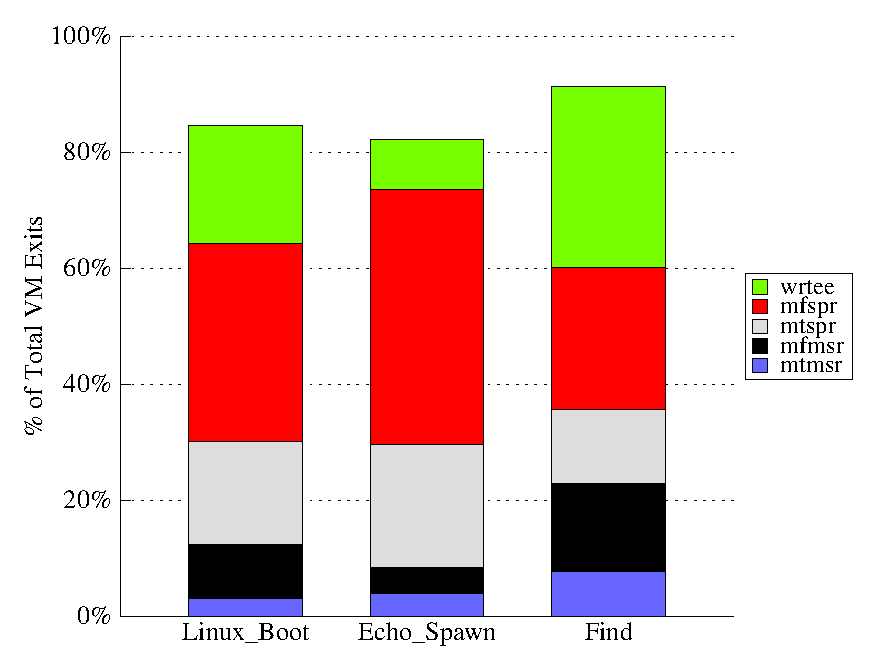
\includegraphics[scale=0.5]{exit_count.eps}
\caption{\label{fig:opcode_exit_fraction}Main sources of VM exits}
\end{figure}

\begin{table}[!b]
\centering
     \begin{tabular}{lcc} \hline
       Instruction class  & Exit count & \% of total exits  \\ \hline
       {\tt mfspr} & 4484245 & 33.8  \\
       {\tt wrtee} & 2792109 & 21.1  \\
       {\tt mtspr} & 2307647 & 17.4  \\
       {\tt mfmsr} & 575302 & 9.5 \\
       {\tt rfi} & 413847 & 4.3 \\
       {\tt mtmsr} & 391813 & 3.1 \\
       {\tt dtlbmiss} & 198239 & 1.5 \\
       {\tt itlbmiss} & 192046 & 1.4 \\
       \hline
     \end{tabular}
\caption{\label{tab:exitcount_linuxboot}Main sources of VM exits and their frequency on guest Linux boot (refer Table~\ref{tab:priv_opcodes} for semantics of these opcodes)}
\end{table}

\begin{table}
\centering
     \begin{tabular}{lcc} \hline
       Exits count  & PC count & \% of total exits  \\ \hline
       $>$20000 & 93 & 91.9  \\
       $>$10000 & 23 & 3.1  \\
       $>$5000 & 68 & 4.2  \\
       $>$2000 & 12 & 0.3 \\
       $>$1000 & 17 & 0.2 \\
       $<$1000 & 299 & 0.2 \\
       \hline
     \end{tabular}
\caption{\label{tab:pcexits_linuxboot}PCs responsible for VM exits on guest Linux boot}
\end{table}

\begin{figure}[!htb]
\centering

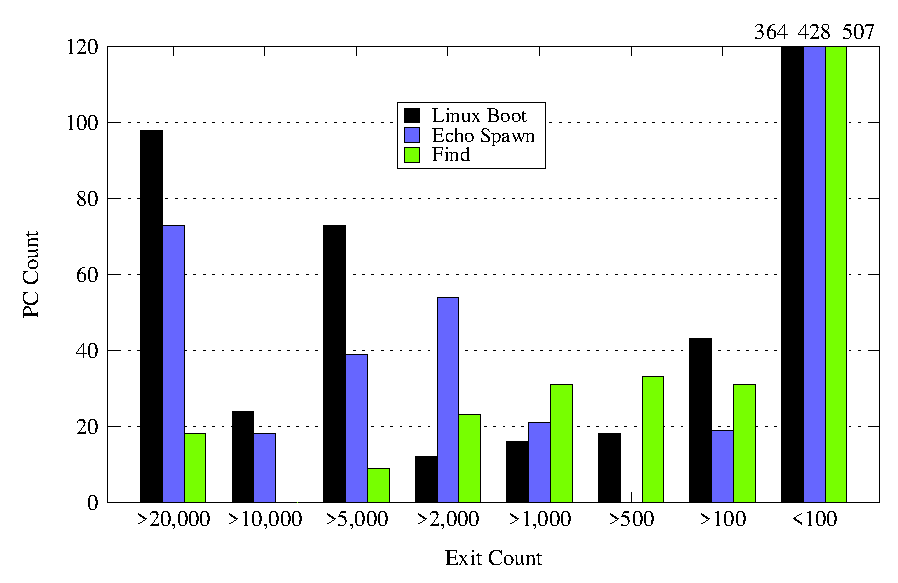
\includegraphics[scale=0.5]{pc_count.eps}
\caption{\label{fig:pc_profile}Exit Profile of Different Guest PCs for three different macrobenchmarks}
\end{figure}

Modifying the guest's address space has obvious pitfalls. Firstly, binary translation must ensure correctness in presence of arbitrary branches in the code. For example, it would be incorrect if the guest could potentially jump to the middle of the translated code.To ensure correctness, a privileged guest instruction is replaced by at most one translated instruction in the guest's address space. Because instructions are fixed length and word aligned on Power Architecture platform, this ensures that there can never be a branch to the middle of the translated code.

These translations to non-privileged VMM logic may be single line  or multi-line in nature. Some privileged opcodes can be emulated by single-instruction translations. For example, {\tt mfmsr} is translated to a {\tt load} instruction to the address of the emulated {\tt msr} register in the shared read/write page. Other opcodes which can be translated to single instructions are {\tt mfmsr}, {\tt mfspr} and {\tt mtspr}. These opcodes requiring single-instruction translations cause the bulk of privileged exits in common workloads (refer Figure~\ref {fig:opcode_exit_fraction}). We call the privileged instruction that was patched, the {\em patch-site}.

Other privileged opcodes require translation to multiple instructions. To implement multi-line translation, such instructions are instead replaced with a direct branch to a emulation code fragment in a host-managed translation cache. Also the emulation code in the translation cache is terminated with another branch {\em back} to the instruction following the patch-site (see Figure~\ref{fig:txcache}). Because each patch-site requires a different terminating branch instruction, a new translation is generated for each patch-site. This branch is  implemented as a single instruction in the guest’s address space, and the translation cache is allocated in host’s address space.

A mechanism for the guest is provided to directly access the translation cache in host’s address space. Thus the translation cache and the emulated guest state must always remain accessible to the translated code in the guest address space for implementing these VMM logics. To allow the guest to directly access the translation cache and emulated guest state maintained by hypervisor, these regions are mapped to an unused/unmapped region of the guest by inserting a shadow tlb entry mapping the guest's unmapped region to these hypervisor maintained structures. Thus the VMM needs to find a large enough unmapped region in the guest’s virtual address space, which can be directly accessed by the replaced instruction. Because a single Power Architecture instruction cannot address the entire 32-bit address space, this places constraints on the placement of these data structures.

We now discuss the resulting placement constraints on these data structures. The translated code needs to access either the emulated guest state or the translation cache.  Single-instruction translations access the emulated state using load and store instructions. To avoid any register overwrites, these memory access instructions must encode the address within the opcode. Power Architecture ISA allows the specification of a signed 16-bit displacement. This implies that the emulated state must lie either in the top or bottom 32KB of the guest address space. If such address space is not available, single-instruction translations can be converted to multiple-instruction translations to allow more placement flexibility.

For multiple-instruction translations, the privileged instruction is replaced with a branch to the translation cache. Branch instructions are of two types: direct and indirect. An indirect branch would clobber the link register or will result in register overwrites. To prevent such clobbering patch multi-line instructions would have to be patched with multi-line translated code which poses the danger of a branch between the translated code as discussed earlier (see Figure~\ref{fig:multiple_insns_patching}). This limits the adaptive binary translator to use direct branches only. A direct branch in Power Architecture platform can only jump $\pm$32MB relative to it's location. This constrains the translation cache to lie within $\pm$32MB of the patch-site.

We found that it is not always possible to find unmapped guest virtual address space which satisfies these constraints. We present a scheme to steal guest’s address space and place these data structures in the stolen space.

\section{Full Adaptive Binary Translation}
\label{full_binary_translation}

\section{Memory Tracing}
\label{memory_tracing}

\begin{figure}[!htb]
\centering

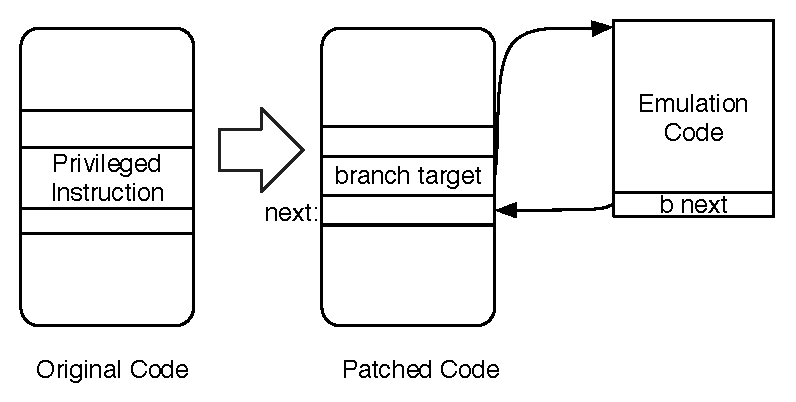
\includegraphics[scale=0.5]{txcache.eps}
\caption{\label{fig:txcache}Figure showing patching of multiple instructions with {\tt branch} instruction.}
\end{figure}

\begin{figure}[!htb]
\centering
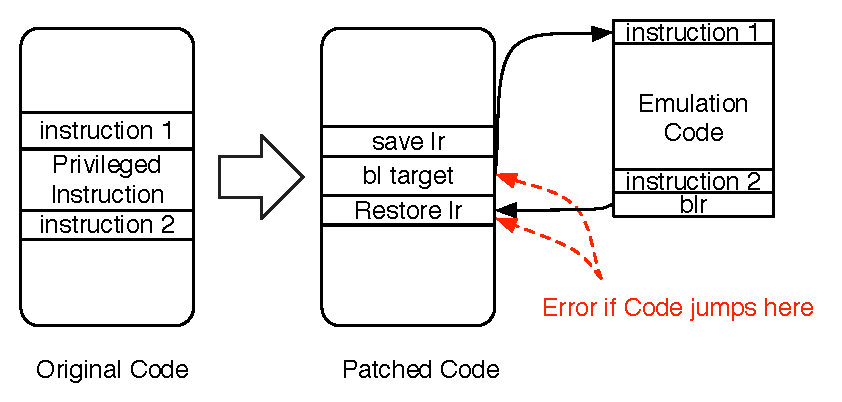
\includegraphics[scale=0.5]{multiple_ins_patching.eps}
\caption{\label{fig:multiple_insns_patching}Figure showing patching of multiple instructions using {\tt bl} instruction. This approach fails in presence of arbitrary guest jumps.}
\end{figure}



\chapter{Read/Write Tracing}\label{ch:3}
\label{sec:memory_tracing}
Adaptive Binary Translation changes the guest address space without the guest knowledge and can cause inconsistencies if the guest tries to read or write this modified code. Thus a mechanism is to be needed in order to make sure the guest's correctness.For this reason, we need to protect the pages containing patch-sites such that whenever the guest accesses anything on these the hypervisor can provide the correct value. Also this protection mechanism should itself be oblivious to the guest to ensure guest's correctness. 

\section{Memory Management in KVM}
\label{memory_management}
In embedded power architecture platforms all modifications to tlb are privilege operations i.e any creation/deletion of a tlb entry by the guest will be trapped by the hypervisor. This mechanism allows the hypervisor to control the guest's MMU to maintain it's isolation and security. In case of KVM for embedded power architecture platforms, the hypervisor creates shadow tlb entries to insert into hardware tlb corresponding to guest tlb entries. Since the guest cannot access the shadow tlb entries directly, as all such accesses will get trapped and emulated by the hypervisor, this provides full flexibility to the hypervisor to choose the sizes and privilege level of the shadow tlb entries. For example hypervisor can use multiple tlb entries to shadow a single guest tlb entry. This mechanism is similar to the hardware-managed shadow page tables used in x86\cite{adams:asplos06}.We implement read/write tracing by disabling read/write privileges in the shadow TLB entries.

\section{Tracing}
Embedded Power Architecture platforms provide three{\tt rwx} protection bits per page for both user/supervisor privilege levels. Using these bits, we can mark a guest page containing a patch site execute-only and removes the read/write permissions from both the supervisor and user privileges. This allows the execution of an instruction on this page to proceed uninterrupted, but any read or write access causes a page fault (and a VM exit). On a page fault, the hypervisor depending on the original privileges levels of the client emulates the faulting instruction in software. We call this method memory read/write tracing (similar to VMware's memory write tracing on x86\cite{adams:asplos06}). 

We implement software emulations of memory instructions in KVM. There are 36 different memory opcodes in Power Architecture ISA that need to be emulated. For read instructions, we simply return the original contents of the memory address in the appropriate destination operand. The original contents may be obtained either from the present guest page (if the address does not intersect with a patch-site), or from the hypervisor's hash table (if the address matches a patch-site), or both. For write instructions, if the memory address (and length) intersects with a patch-site, we invalidate and free the corresponding translation cache entry and replace the guest page with it's original contents before re-executing the instruction. If the memory address does not intersect with a patch-site, we simply perform the equivalent write operation to the guest's memory. 

The overhead of read/write tracing depends on the number of accesses by the guest to its pages containing kernel code. For a Linux guest, we found that this overhead can be quite significant. Much of this overhead is due to false sharing. For example, a large number of page faults occur because guest kernel data often resides on the same page as guest kernel code. The problem becomes worse with increasing page size. Also a large page may span both the text/code section as well as the data section of the kernel resulting in every access to that data section into a VM exit. Linux on embedded Power Architecture platform uses huge pages for kernel code/data to minimize TLB pressure, causing our tracing mechanism to result in a huge number of page faults. We call these {\em tracing page faults}. We discuss our optimizations to reduce these tracing page faults in Section~\ref{sec:tracing_optimizations}.

This mechanism of read/write tracing gives us an early stage solution to virtualization on Powerpc Embedded Architecture platforms. Though the tracing page faults may even downgrade the performance to even less than the native KVM, but it is to be noted that it guarantees the fidelity of the guest's execution with binary translation optimizations to be exact as before the binary translation optimizations.




\chapter{Shared spaces}\label{ch:4}
\label{sec:shared_space}

Shared address space between the hypervisor and the guest is used for implementing the VMM logic of translations during adaptive binary translations. Two different types of shared space are required for performing adaptive binary translation. One is used to store the emulated state of the guest as maintained by the hypervisor. All privileged opcodes that are being patched i.e mfmsr,mfspr, mtspr, mtspr, wrtee (for details please see Table~\ref{tab:priv_opcodes}) in general are trying to modify the guest execution state. Such instructions are accessing or modifying some privilege register maintained by the hypervisor. This memory region is used to store all such emulated registers to maintain the guest emulated state and is shared between the guest and the hypervisor. All privilege instructions are patched with translation code to modify these emulated state registers directly from the shared space thus saving VM exits. These translations may be single line or multi-line in nature as discussed in Section~\ref{adaptive_binary_translation}. The other shared address space called translation cache comes into action while implementing such multi-line translations. Translation cache contains the emulation code for translations requiring multi-line instructions to implement the VMM logic. Also this shared space also has constraints that it should lie within $\pm$32MB of the patch-site.

\section{Setup}
\label{setup_space}
As discussed in Section~\ref{adaptive_binary_translation} the shared space sharing the guest emulated state is constrained to be either in top or bottom 32KB of the guest's address space if single line translations are allowed. In Linux we use the top address space of the guest to map this address space. To make sure that this address space is not being used we keep track of the guest tlb entries mapping the guest address space. If any guest tlb entry is found to map this region then single line translations are removed and the emulated guest's state will be stored at any another unmapped guest's region and can be accessed using multi-line translation. If no such unmapped region is found then the binary-optimizations are not done.

Translation cache is required to store the translations for multi-line patching and is constrained to be within $\pm$32MB of all such patch-site. In practice we needed a translation cache of as small as 32KB for containing all the multi-line translations. To met these requirements we steal some region from the guest address space to create space for the translation cache. The stolen space from the guest's address space must belong to a data section since any branch or in-between jump to translation cache by the guest without our knowledge will result in an unexpected behavior. Thus a region belonging to a data section will be sure not to have such jumps and in-between branches. The kernel’s read-only, read-write data, and bss sections are examples of such data sections. If a 32KB or larger data region is available within ±32MB of the patch-site, we steal 32KB from this region and copy it to the host, and use this region’s space to store the translation cache(see Figure~\ref{translation_cache_stealing}). This region is then marked execute-only so that all original accesses to this region now trap into the hypervisor and emulated correctly. This presents us a mechanism to dynamically allocate the translation cache without guest's knowledge while ensuring the guest's correctness.

Stealing a region from a data section increases the tracing page faults on this stolen region which further deteriorates our optimization performance since the data section can be heavily accessed region and every such access is trapped and needs to be emulated. These tracing page faults can degrade the performce results due to binary optimizations and need to be optimized. We discuss our optimization to reduce these tracing page fualts in Section~\ref{tcache_optimizations}. 

The other way of acquiring translation cache is to get it allocated by the guest and the guest will inform the host using a hypercall mechanism. This requires static changes in the guest kernel similar to para-virtual extensions and thus are not used.






\chapter{Tracing Optimizations}\label{ch:5}
Read/write tracing is used to correctly emulate self-referential and self-modifying code in the guest, and to steal guest data address space for the translation cache. Tracing results in extra page faults, and these page faults can result in significant performance degradation. In fact, without any optimizations, the number of such page faults is far greater than the number of exits caused due to privileged instructions in unmodified KVM running a Linux guest.
We implement two optimizations to reduce tracing page faults. Our first optimization adaptively resizes the guest’s pages to reduce false sharing. Our second optimization adaptively mirrors guest data (which is causing a large number of faults) to reduce the number of page faults caused by read accesses (which is the common case). For the second optimization we also translate the faulting instruction to access the mirrored data. We discuss both optimizations in detail below.

\section{Adaptive Page Resizing}
Typical TLB sizes on embedded Power Architecture processors are small. For example, the software-managed TLB on our test system is a combination of a 16-entry fully-associative cache of variable-sized page table entries and a 512-entry 4-way set-associative fixed-size (4KB) page table entries. A faster L1 TLB lookup cache is implemented in hardware, and all invalidations to maintain consistency with the software-programmed L2 TLB are done automatically. The variable-pagesize TLB cache supports 11 different page sizes: 4K, 16K, 64K, 256K, 1M, 4M, 16M, 64M, 256M, 1G, and 4G. Further a page of size S must be S-byte aligned in physical and virtual address spaces.

As explained in Section~\ref{memory_management} the hypervisor has full flexibility to control the shadow tlb entries for mapping the guest tlb entries. It can even map multiple shadow entries corresponding to a single guest tlb entry. To minimize TLB pressure, the hypervisor typically uses one shadow TLB entry per guest TLB entry. For example, if the guest uses 4MB pages, then the shadow TLB will also have corresponding entries for 4MB pages. Most operating systems use huge pages (using the variable pagesize TLB cache) for the kernel to reduce TLB pressure. The fixed pagesize TLB cache (containing map- pings for 4K pages) is made available primarily for user programs. For example, our Linux guest uses just one 256MB TLB entry mapping all its kernel code and data. Disabling read/write privileges from this TLB entry predictably causes an unacceptably large number of page faults (every kernel data access becomes a page fault).

Most of tracing faults are due to the false sharing as a result of the huge pages used by the OS. The problem can be avoided/reduced by resizing the shadow tlb entries into smaller entries to reduce tracing page faults due to read/write tracing. This will reduce false sharing resulting in less of the data section to be traced and a less number of tracing page faults. Also breaking a shadow tlb entry into multiple entries leads to increased tlb pressure and an increase in tlb misses again degrading the performance. Thus page resizing essentially is a tradeoff between the tracing page faults and increased tlb pressure.

We resize shadow TLB entries to deal with this overhead of page faults due to read/write tracing. While patching a guest privilege instruction, if the shadow tlb entry for the page containing this patch-site is not already traced and this patch-site is contained in a huge page, then the page (and the corresponding shadow tlb entry) containing this patch-site is fragmented into smaller entries such that the entry contining the patch-site is atmost 1MB large. Also on a traced page, if we notice a high number of tracing page faults on that page, we break the page into smaller fragments (and the corresponding TLB entry into smaller TLB entries). To minimize false sharing, we keep the size of the page containing the patch-site as small as possible, without adversely effecting performance. All other pages created by this fragmentation are sized as large as possible, to minimize the overall number of TLB entries. While smaller pages reduce false sharing, they also result in increased TLB pressure.

Breaking a large page potentially creates many smaller pages due to alignment restrictions. For example, if the kernel has mapped itself using a 256MB page at virtual address (0xc0000000,0xcfffffff), and a patch is to be applied at address 0xc0801234, and we have decided to break the patch-site page into a 4MB page, the new set of TLB entries will be for addresses (0xc0000000, 0xc03fffff); (0xc0400000, 0xc07fffff) (0xc0800000, 0xc0bfffff); (0xc0c00000, 0xc0ffffff); (0xc1000000, 0xc1ffffff); (0xc2000000, 0xc2ffffff); (0xc3000000, 0xc3ffffff); (0xc4000000, 0xc7ffffff); (0xc8000000, 0xcbffffff); (0xcc000000, 0xcfffffff). Notice that each page of size S is S-byte aligned and S is always one of the values supported by the architecture. Thus fragmentation of a single entry in this case has lead to 10 smaller shadow entries resulting in an increase in tlb pressure and tlb misses.

If a large number of tracing page faults are noticed on a page smaller than 64KB, then instead of fragmenting it further we remove all the patch-sites from this region and re-instate it's original read/write permissions. This is done in order to prevent the tlb thrashing which results due to excessive fragmentation of a tlb entry. This decision on whether to remove the patch-sites also depends on tradeoff between the number of privileged instruction exits due to privilege instructions on this page and the tracing page faults experienced at that point of guest's execution.

On noticing a large number of tracing page faults on a traced page, we fragment it into smaller pages to reduce false sharing. The fragmentation policy needs to be different for different profiles of tracing page faults. We use two different policies in our implementation depending on the nature of page faults. Typically page faults either occur in bursts (a large number of faults occur on a  small set of closely-located addresses on a single large page) or in scans (faults are spread over a large region with a small number of faults per address). for e.g if a data section get's traced due to false sharing, we generally observe bursts of accesses on such regions while examples of scan are during the self modifying behavior of the guest. 

For bursts, the ideal way to resize the pages is to detect the region in the page where the page faults are concentrated and resize the page such that the page faults belong to a single smaller tlb entry and then untrace this entry. This smaller entry should be kept as small as possible (without thrashing the tlb too much) since there is tradeoff between the privileged exits on this region and the page faults. We use a threshold of 20000 tracing page faults within 100ms to detect the need for page resizing. If these faults are concentrated in a small region then a burst has been deteced and we resize this page such that the concentrated page fualts belong to a 64KB page and trace is removed form this page and the corresponding patch-sites are removed. For scans, where the tracing page faults are distributed across a large address range, the page is broken into two halves (4 shadow tlb entries) and the half with larger number of tracing page faults is untraced. We do this only if the number of tracing page faults is greater than threshold $T$ of this page. 

Also if a region has been untraced earlier due to either a burst or scan detected on that region, it can be traced again as soon as the number of privilege exits on this region are greater than the threshold T of this page. These conversion from traced to untraced and vice-versa may lead to tlb thrashing due to continuous fragmentation of the pages. To resolve this we opportunistically merge the pages to larger pages after every periodic interval (100ms in our implementation). If we find pages with similar {\tt rwx} privileges we merge them to form a larger page (shadow entries for these pages might merge or not since the combined size of these pages might not be supported on the system). This opportunistically merging helps in reducing the tlb pressure and thus improves the performance.

The threshold $T$ is determined dynamically, as it depends on the tradeoff between the number of privileged instruction exits and tracing  page faults on that page. On tracing a page, we record the number of privileged instruction exits that this page was experiencing, before it got patched and traced. This serves as our threshold $T$ for that page. If the number of tracing page faults we are experiencing on this page is greater than $T$, we untrace it by removing all it's patches. On each tracing or untracing event on a page, the threshold $T$ is updated and is used to determine whether to again trace or untrace the page during future execution. Hence, after a page is untraced, $T$ is also used to determine whether to retrace it or not (we retrace if the number of privileged instruction exits > $T$).

Our dynamic thresholding mechanism relies on the assumption that the expected number of privileged instruction exits (or page faults) after  untracing (or after re-tracing) will be similar to what had been observed previously. If the guest has time-varying behaviour, it can result in bad decision-making and consequently performance penalties. For example, a guest may execute a privileged instruction a large number of times in the beginning and then never execute it again. This may result in T being raised to a large value in the beginning causing the page to remain traced unnecessarily, and thus resulting in tracing page faults that could have been avoided. To avoid such situations, our threshold T decreases linearly with time at the rate of 2000 per 100 ms. 

Adaptive page resizing significantly reduces the number of page faults. It uses the spatial and time locality of the privileged exits and tracing page faults to trace/untrace a region or to patch/unpatch a page. For example, a Linux guest boots in 13.03 seconds (as opposed to 30.03 seconds on unmodified KVM) with in-place binary translation and adaptive page resizing for read/write tracing. Without adaptive page resizing, the guest livelocks at boot time due to the large number of page faults. A detailed study of the performance tradeoffs is presented in Section~\ref{sec:results}.

\section{Adaptive Data Mirroring}
\label{adaptive_dm}
Adaptive page resizing profiles the exits both thr privilege exits and tracing page faults and tries to pick the best at the cost of other. Thismechansim works well when the privilege text and data sections are far apart but fails when they are close enough and both of them are frequently used. For example the function dispatch tables and the exception handlers are located within the kernel text section and resides close (within 64KB region of it) to the privileged text accessing them. Both of them are frequently executed and accessed causing the adaptive page resizing algorithm perform bad due to increase in the tlb pressure. We can observe a 10-20\% performance overhead in Table~\ref{tab:detailed_results}. 

We avoid these faults by dynamically monitoring such tracing page faults, adaptively copying the data being accessed to the shared space between the host and the guest and translating the instructions to access them from their new location. This optimization prevents furter page faults on this data. 

We perform this optimization if the number of tracing page faults due to a certain read-access instruction exceeds a threshold (we use a threshold of 200 accessess). On noticing such faults, we copy the data being accessed to a “data cache”. This data cache is maintained in the read/write shared page also storing the guest’s emulated registers. The faulting instruction is replaced with code to check the data cache for the address being read. If the check succeeds, the translated code reads the data from the cache, thus avoiding a page fault. If the check fails, the translated code executes the original instruction just as before (which may result in a page fault just as before). If the hit rate of the data cache is high, we have reduced the number of page faults. This translation code of the fault- ing instruction is stored in the translation cache (maintained in the execute-only shared space) and the faulting instruction is replaced with a branch to this code. 
To maintain guest correctness, the pages containing patches for faulting instructions (due to tracing) need to be read/write traced too. This can potentially result in a chain-effect: tracing of these new pages can cause more tracing page faults, resulting in more pages to be patched and traced, resulting in more tracing page faults, and so on\ldots. Fortunately, we do not see this chain effect in practice. The faulting instructions that are patched typically reside on a page that is already being traced, causing this cycle to converge on the first iteration. Even if the patching of the faulting instructions requires a new read/write trace to be created, we expect this cycle to converge in 1-2 iterations. Intuitively, kernel code which causes privileged VM-exits or tracing page faults is likely to be spatially close, and will eventually lead to a small set of traced pages. We observed this behaviour in all our experiments with Linux guests. Even if the read write tracing chain becomes long, we rely on our adaptive page resizing algorithm to break this chain by removing the trace on a page (and all the associated patch-sites) if that page experiences a large number of page faults. 

Finally, we note that this optimization is also valid for write accesses. For write accesses, we translate the instruction to access the  mirrored data location directly. Other instructions trying to read/write the original data instruction trap and get emulated (or translated, if this happens frequently). All we need to make sure during the write accesses is that if the data we have mirrored is a text which can be executed, then we need to flush the contents of the data cache maintained by us at their corresponding data cache flush.

\section{Optimizing Translation Cache}
\label{tcache_optimizations}
As disscussed in Section~\ref{setup_space} stealing translation cache from data segment of the guest degrades the performance since the data sections are generally heavily accessed and every such access will result in a VM exit. For example when the initial aligned 64KB of address space is stolen from the guest {\tt RO} segment for translation cache the linux boot benchmark experiences around 1,000,000 exits due to tracing page faults which itself is pretty large number and might even increase/decrease if the space is stolen from other regions. Adaptive Data Mirroring it to data cache maintained in the shared space as discussed in the last section will also not be too effective since this region is data section and the accesses are typically widespread resulting in a large number of cache misses and thus tracing page faults. Also page resizing cannot be used to reduce page faults since we cannot remove trace from this region since this shared space needs to be traced permanently as long as binary translation optimizations are active.

In order to optimize these page faults we can mirror the original contents of the stolen space in a shared address space with the guest. This shared address space is similar to the address space used to store the emulated guest space i.e region that is not mapped/used by the guest. In other words we have increased the size of the first shared address space to be equal to the size of the stolen region for translation cache and the space used to store the emulated state of the guest. In our implementation we have used the top most region of the Linux Guest which was not being used to map this region. All instructions accessing the stolen regions are now translated similar to the case of data mirroring to access the mirrored section directly and thus avoiding page faults. If no such unmapped region is found in the guest then this optimization is not done. Table~\ref{tab:tcache} compares the results of the case when the translation cache has been allocated by the guest with the cases when we are stealing address space from the guest for storing translation cache with/without the forementioned optimizations.

\begin{table*}
\centering
      \begin{tabular}{|l| p{3.1cm} |p{3.1cm}|p{3.1cm}|} \hline
        Benchmark\verb, ,& {\tt Guest allocated Tcache} \verb, ,& {\tt Stolen} \verb, ,& {\tt Stolen \& optimized} \verb, , \\ \hline

     & \multicolumn{3}{c|}{Running Time in $sec$}\\ \cline {2-4}
Linux boot	&	12.24	&	14.39	&	12.39	\\
Echo Spawn	&	7.26	&	8.90	&	6.85	\\
Find	&	0.67	&	1.67	&	0.83	\\
Lame	&	0.51	&	0.50	&	0.50	\\
\hline
      \end{tabular}
\caption{\label{tab:tcache}Measuring the overhead and performance when translation cache is allocated by guest, in comparison to a when translation cache is being stored in stolen space but without any optimizations and when translation cache is being stored in stolen space with data mirroring optimizations.}
\end{table*}









\chapter{Experimental Results}\label{ch:6}
We implement our optimizations in Linux/KVM version 3.0, which has paravirtual extensions for Power. To measure performance of {\em unmodified} KVM and KVM with our optimizations, we disabled the paravirtual extensions. We perform our experiments on Freescale QorIQ P2020 platform, which is optimized for single-threaded performance per watt for networking and telecom applications. Our system has a 1.2GHz processor with 32KB L1 cache and 512 KB L2 cache. We use RAMdisk for our experiments to eliminate I/O overheads.

Our benchmarks are described in Table~\ref{tab:kvm_performance}. We use four macrobenchmarks, namely Linux boot, Echo spawn, Find and Lame. These benchmarks have also been used in a previous performance study\cite{kvm_ppc_exittimings}. The others are microbenchmarks from the widely-used {\tt lmbench} toolset\cite{lmbench} and {\tt unixbench} toolset \cite{unixbench}. Linux boot and Echo spawn execute a large number of privileged instructions, while Find executes relatively fewer privileged instructions. Lame has to do some IO and a lot of computation that does not need to exit to the hypervisor, thus representing an average compute-intensive workload. 

{\tt Lmbench} is a performance analysis suite of micro-benchmarks for UNIX/POSIX. The microbenchmarks are designed to provide the latency and bandwidth deatils of diferent system operations. The microbenchmarks are extensible in nature and target specific subsytems and operations to measure hardware performances for example fork benchmark targets the performance anlaysis of process creation only.

{\tt Unixbench} is also a benchmarking suite to analyze the system performances of Unix-like systems. It also contains the microbenchmarks to test various aspects of system performance. These micro-benchmarks are also specific in nature and targets different subsytems of the system. A major difference with the lmbench benchmarking suite is that while lmbench suite provides the latency of the different subsystems it can't be used to compare the tlb misses, privileged exits and tracing page faults since the number of executions of the micro-benchmark depends on the latency of the benchmark itself. The Unixbench microbenchmarks can be tunes to execute the benchmarks for a fixed number of times giving more coorect data about the overheads and performance optimizations due to adaptive binary translation and tracing.

The number of privileged instructions executed by each benchmark are reported in Table~\ref{tab:vm_exit_stats}. We do not report performance comparisons on purely user-level compute-intensive workloads because they exhibit near bare-metal performance for all cases.

\section{Comparison of native with various virtualization solutions}
We implement the following optimizations in Linux/KVM:
\begin{enumerate}
  \item In-place Binary Translation and Read/Write Tracing
  \item Adaptive Page Resizing
  \item Adaptive Data Mirroring and Translation of Faulting Instructions
\end{enumerate}
Table~\ref{tab:detailed_results} summarizes our performance results before and after these optimizations. Different workloads show different improvements. The improvement primarily depends on a three-way tradeoff between the number of VM exits due to privileged instructions, the number of tracing page faults, and the number of page faults due to increased TLB pressure (TLB misses). Table~\ref{tab:vm_exit_stats} shows the number of VM exits and page faults due to all these three reasons for each workload, before and after our optimizations. We also show the number of exits in the paravirtual solution ({\tt KVM-PV}) for comparison. The number of exits in {\tt KVM-PV} can be considered as a lower-bound on the number of exits achievable by a host-side binary translation solution.

Just using Optimization 1 does not improve performance for a Linux guest. In fact, we find that read/write tracing severely impairs performance because the guest uses a huge 256MB page to map the kernel's code and data. If we constrain the host to only use 4KB shadow pages, the performance improves but is still unacceptably low due to high TLB pressure.

\begin{table*}
\centering
      \begin{tabular}{|l| r r r |} \hline
        Benchmark\verb, ,& {\tt KVM} \verb, , & {\tt Adapt-PR} \verb, , & {\tt Adapt-DM}  \\ \hline
     & \multicolumn{3}{c|}{ Running Time in $sec$}\\ \cline {2-4}  
Linux boot	&	30.03	&	13.02	&	12.39	\\
Echo Spawn	&	21.34	&	7.80	&	6.85	\\
Find	&	1.89	&	0.98	&	0.83	\\
Lame	&	0.56	&	0.51	&	0.50	\\
\cline{2-4}
	   
     & \multicolumn{3}{c|}{Latency in $msec$}\\  \cline{2-4}
syscall	&	0.020	&	0.009	&	0.003	\\
stat	&	0.033	&	0.012	&	0.007	\\
fstat	&	0.021	&	0.009	&	0.004	\\
open/close:	&	0.067	&	0.026	&	0.023	\\
sig hndl	&	0.024	&	0.009	&	0.004	\\
pipe 	&	0.066	&	0.062	&	0.041	\\
fork	&	6.641	&	2.020	&	1.679	\\
exec	&	20.543	&	7.457	&	6.681	\\
sh	&	45.164	&	16.567	&	14.719	\\
 \hline
\cline{1-4}
\multicolumn{1}{|c|}{Unixbench Benchmark}     & \multicolumn{3}{c|}{Number of Calls}\\  \cline{1-4}
Dhrystone 2	&	48110141	&	48904947	&	48957180\\
System Call	&	124854	&	286057	&	652829\\
Pipe-based context switching	&	60746	&	159256	&	240653\\
Process Creation	&	2470	&	7679	&	8714\\
Pipe Throughput	&	188208	&	469538	&	923218\\
Hanoi	&	8689401	&	8690019	&	8836219\\
\cline{1-4}
\multicolumn{1}{|c|}{Unixbench Filesystem Benchmark}     & \multicolumn{3}{c|}{Throughput in KBps with 256 bufsize and 2000 max blocks
}\\  \cline{1-4}
File Read	&	11524	&	24151	&	49830\\
File Write	&	10500	&	19050	&	38200\\
File Copy	&	5432	&	10408	&	20070\\	\cline{1-4}

      \end{tabular}
\caption{\label{tab:detailed_results}Performance Improvements obtained by Adaptive Page Resizing ({\tt Adapt-PR}) and Adaptive Data Mirroring ({\tt Adapt-DM}) optimizations.}
\end{table*} 

\begin{center}
\begin{table*}
\centering
\begin{tabular}{
  |p{1.2cm}@{}|@{ }c@{ }|@{}p{0.9cm}|@{}p{1.2cm}|@{}p{1.0cm}@{}|@{ }c@{ }|@{}p{0.8cm}|@{}p{1.2cm}|@{}p{1.0cm}|@{ }c@{ }|@{}p{0.8cm}|@{}p{1.2cm}|@{}p{0.9cm}|@{ }c@{ }|@{}p{0.8cm}|@{}p{1.2cm}|@{}p{0.9cm}@{}|} \hline
	         &  & \multicolumn{3}{c|}{\tt KVM}& & \multicolumn{3}{c|}{\tt Adapt-PR} & & \multicolumn{3}{c|}{\tt Adapt-DM} & & \multicolumn{3}{c|}{\tt KVM-PV} \\ \hline

           &&{\tt Priv. Exits}&{\tt TLB miss}&{\tt Acc. Viol} &&{\tt Priv. Exits}&{\tt TLB miss}&{\tt Acc. Viol.}&&{\tt Priv. Exits}&{\tt TLB miss}&{\tt Acc. Viol}&&{\tt Priv. Exits}&{\tt TLB miss}&{\tt Acc. Viol} \\ \hline  
Boot	&&	11509859	&	402274	&	13823	&&	48560	&	326825	&	460001	&&	38367	&	345035	&	77467	&&	40451	&	295672	&	14181	\\	\hline
Find	&&	802777	&	2485	&	46	&&	965	&	2655	&	98145	&&	851	&	2782	&	4701	&&	719	&	2392	&	46	\\	\hline
Lame	&&	60312	&	1932	&	23	&&	636	&	2085	&	3126	&&	644	&	2114	&	46	&&	625	&	1916	&	24	\\	\hline
Echo Spawn	&&	9829128	&	419191	&	18005	&&	35823	&	492129	&	518255	&&	35014	&	506295	&	18624	&&	34602	&	427351	&	17011	\\	\hline
Pipe 	&&	28714485	&	979	&	41	&&	18762	&	1113	&	6010468	&&	9185	&	1165	&	75	&&	7648	&	968	&	42	\\	\hline
Hanoi	&&	4005414	&	914	&	40	&&	225211	&	1088	&	151308	&&	224970	&	1169	&	876	&&	224660	&	943	&	41	\\	\hline
Syscall	&&	22541901	&	953	&	41	&&	15105	&	1130	&	6008149	&&	6324	&	1159	&	40	&&	5197	&	948	&	41	\\	\hline
Process Creation	&&	19841882	&	621658	&	60036	&&	100796	&	835408	&	897302	&&	99081	&	846053	&	60026	&&	98569	&	652042	&	60034	\\	\hline
Context switching	&&	26459239	&	1102	&	49	&&	616684	&	7702	&	3609690	&&	610986	&	5567	&	49	&&	608549	&	1059	&	49	\\	\hline
Dhrystone 2	&&	154460	&	973	&	40	&&	7656	&	1127	&	6132	&&	7648	&	1140	&	38	&&	7667	&	1001	&	40	\\	\hline
      \end{tabular}
\caption{\label{tab:vm_exit_stats}Frequency of VM exits due to privileged instructions ({\tt Priv. Exits}), TLB misses ({\tt TLB miss}), and access violations ({\tt Acc. Viol}). The
exits due to access violations are due to read/write accesses to pages which do not have read/write permissions. These exits occur primarily due to read/write tracing.}
\end{table*} 
\end{center}


Optimization 2 adaptively resizes the shadow TLB entries to reduce the number of tracing page faults and results in performance improvements over unmodified KVM. The second column ({\tt Adapt-PR}) in Table~\ref{tab:detailed_results} shows the performance of KVM with Optimizations~1~and~2. We first discuss the {\tt lmbench} microbenchmarks. The running time of all microbenchmarks improves with Optimizations~1~and~2. The average improvement is 148\%, with the maximum improvement of 223\% in fork. The improvement in a benchmark primarily depends on the reduction in the number of privileged exits. Different microbenchmarks execute different number of privileged instructions and show different corresponding reductions. We next discuss the improvement on macrobenchmarks using Optimizations~1~and~2. We observe a performance improvement of 101\% on the macrobenchmarks, with the maximum improvement seen in Echo Spawn, which also shows the maximum reduction (99\%) in exits due to privileged instructions. For {\tt unixbench} microbenchmarks, the average improvemnt is XX\%, with maximum improvement in XX. 

For both microbenchmarks and macrobenchmarks, we notice an increase in the number of TLB misses and access violations (due to tracing page faults) on average. The net effect however remains positive. Our next optimization (Optimization~3) further reduces these access violations. We also find that Optimization~3 reduces privileged instruction exits. A slight increase in tlb misses can be observed after Optimization~3 this is due to the fact that in the solution obtained from Optimization~1~and~2  the translation cache is being allocated by the guest while with Optimization~3 steals it from the data section causing a slight increase in the tlb misses. Also since the translation cache is being allocated by the guest using paravirtual extensions in the guest in solution obtained from Optimization~1~and~2, the scan behavior of the guest while dynamically modifying it's guest is not visible while with Optimization~3 this behvior causes the page resizing algorithm to kick in and results in an increase in tlb misses to save tracing page faults.
This increase has been subdued due to an indirect effect, without Optimization~3 certain guest pages are broken into smaller pages and some of these smaller pages are removed to reduce tracing page faults. With Optimization~3, the number of tracing page faults decreases. This allows Optimization~2 to not have to kick in, allowing pages to remain unbroken and privileged instructions to remain patched. This subdues the TLB misses and also reduces the number of privileged instruction exits. 

Optimization~3 reduces the number of tracing page faults by mirroring the data residing on a traced page and patching the corresponding access instruction to access the data from the mirrored location in future. The reduction is observed in all our benchmarks. The average reduction in the number of access-violation page faults (which are mostly due to tracing page faults) is XX\%.

Overall Optimizations~1,~2~and~3 provide performance comparable to paravirtualization. On our macrobenchmarks, we observe an average speedup of XX\% over unmodified KVM. Optimization~3 provides significant improvements on many benchmarks, including the {\tt find} macrobenchmark, where the improvement is around XX\%. Table~\ref{tab:vm_exit_stats} confirms that these improvements are due to the reduction in exits caused by tracing page faults, and privileged-instruction executions.

\section{Static TLB configured Guest vs Adaptive Page Resizing}
We next measure the overhead and effectiveness of our adaptive page resizing algorithm. We statically configured the shadow TLB to the best observed configuration for Linux boot benchmark. In this configuration, we loaded the shadow TLB with 13 entries: one entry of size 4MB ({\tt 0xc0000000-0xc03fffff}), four entries of size 1MB each (covering {\tt 0xc0400000-0xc07fffff}), two entries of size 4MB each (covering {\tt 0xc0800000-0xc0ffffff}), three entries of size 16MB each (covering {\tt 0xc1000000-0xc3ffffff}), and three entries of size 64MB each (covering {\tt 0xc4000000-0xcfffffff}). Of these 13 entries, the first two entries were marked execute-only (kernel code is nearly 5MB long) and the rest remained unmodified. We compared the performance of this configuration with our adaptive page resizing algorithm. We disabled Optimization~3 ({\tt Adapt-DM}) for this experiment. Table~\ref{tab:adaptive_tlb_resizing} summarizes our results. For Linux boot benchmark, we observe that our resizing algorithm performs within 1-2\% of the optimal and within 10-20\% of all the other microbenchmarks as well as macrobenchmarks.

The adaptive-pr solution soon approaches the static configuration as it starts patching the privilege instructions. The tracing page faults we observe in Table~\ref{tab:adaptive_tlb_resizing} are mainly due to the accesses to function dispatch tables and exception handlers. As explained in Section~\ref{adaptive_dm} the adaptive page resizing algorithm keeps on trying to break the shadow tlb entries in order to reduce the trace page faults but has to revert back since the privileged code section accessing these are co-existing with them and are equally frequent. this leads to a slight increase in the tlb misses. 

A more fitting benchmark would be when some data section which is heavily accessed got included in a traced region. {\tt Custom Pipe} and {\tt Custom Syscall} are custom experiments where all the privileged code belonging accessing the exception handlers and function dispatch tables has been removed statically from the guest and {\tt Pipe} \& {\tt Syscall} from unixbench are run on it. Thus the memory region containing the function dispatch tables and exception handlers now act as nearly pure data section. We can observe a 30x decrease in number of tracing page faults in both these custom experiments. An increase in tlb misses can be observed also due to fragmentation but the increase in terms of absolute tlb misses is not so significant as compared to the decrease in exits due to tracing page faults. The same behavior is reflected in their raw scores for these custom experiments.

\begin{table*}
\centering
      \begin{tabular}{|p{2.0cm}| r r |} \hline
        Benchmark\verb, ,& {\tt Static-TLB} \verb, ,& {\tt Adapt-PR} \verb, , \\ \hline

     & \multicolumn{2}{c|}{Running Time in $sec$}\\ \cline {2-3}
Linux boot	&	12.98	&	13.02\\
Echo Spawn	&	8.0	&	7.80\\
Find	&	0.90	&	0.98\\
Lame	&	0.51	&	0.51\\
\cline{1-3}
\multicolumn{1}{|c|}{Lmbench Benchmark}     & \multicolumn{2}{c|}{Latency in $msec$}\\  \cline{1-3}
syscall	&	0.007	&	0.009\\
stat	 &	0.011	&	0.012\\
fstat	&	0.008	&	0.009\\
open/close:	&	0.022	&	0.026\\
sig hndl	&	0.008	&	0.009\\
pipe 	&	0.053	&	0.062\\
fork	&	2.068	&	2.020\\
exec	&	7.792	&	7.457\\
sh	&	17.076	&	16.565\\
\cline{1-3}
\multicolumn{1}{|c|}{Unixbench Benchmark}     & \multicolumn{2}{c|}{Number of Calls}\\  \cline{1-3}
Dhrystone 2	&	48833854	&	48904947\\
System Call	&	344877	&	286057\\
Pipe-based context switching	&	160575	&	159256\\
Process Creation	&	7101	&	7679\\
Pipe Throughput	&	557045	&	469538\\
Hanoi	&	8835343	&	8690019\\
Custom Pipe	&	557045	&	994777\\
Custom Syscall	&	344877	&	739343\\
\cline{1-3}
\multicolumn{1}{|c|}{Unixbench Filesystem Benchmark}     & \multicolumn{2}{c|}{Throughput in KBps with 256 bufsize and 2000 max blocks
}\\  \cline{1-3}
File Read	&	28346	&	24151\\
File Write	&	22450	&	19050\\
File Copy	&	12201	&	10408\\
 \hline
      \end{tabular}
\caption{\label{tab:adaptive_tlb_resizing}Measuring the overhead and performance of adaptive page resizing ({\tt Adapt-PR}) algorithm, in comparison to
a statically configured TLB ({\tt Static-TLB}). The static TLB configuration was setup such that it provides the best performance for the Linux boot benchmark. We disable {\tt Adapt-DM} optimization for this experiment.}
\end{table*} 

\begin{table*}
\centering
\begin{tabular}{|l|@{ }c@{ }|p{1cm}|c|p{1cm}|@{ }c@{ }|p{1cm}|c|p{1cm}|} \hline
	         &&  \multicolumn{3}{c|} {Static TLB Configuration}&& \multicolumn{3}{c|} {Adapt-PR} \\ \hline

           &&{\tt Priv. Exits}&{\tt TLB miss}&{\tt Acc. Viol}&&{\tt Priv. Exits}&{\tt TLB miss}&{\tt Acc. Viol}\\ \hline  
Boot	&&	41770	&	320941	&	452482	&&	48560	&	326825	&	460001	\\	\hline
Find	&&	908	&	2676	&	98113	&&	965	&	2655	&	98145	\\	\hline
Lame	&&	637	&	2052	&	3124	&&	636	&	2085	&	3126	\\	\hline
Echo Spawn	&&	35929	&	485870	&	513294	&&	35823	&	492129	&	518255	\\	\hline
Pipe 	&&	15742	&	1144	&	6008821	&&	18762	&	1113	&	6010468	\\	\hline
Hanoi	&&	224929	&	1116	&	151104	&&	225211	&	1088	&	151308	\\	\hline
Syscall	&&	12791	&	1135	&	6006963	&&	15105	&	1130	&	6008149	\\	\hline
Process Creation	&&	101427	&	815074	&	897920	&&	100796	&	835408	&	897302	\\	\hline
Context switching	&&	614104	&	1260	&	3608524	&&	616684	&	7702	&	3609690	\\	\hline
Dhrystone 2	&&	7663	&	1197	&	6158	&&	7656	&	1127	&	6132	\\	\hline
Custom Pipe	&&	15742	&	1144	&	6008821	&&	15832	&	63963	&	235367	\\	\hline
Custom Syscall	&&	12791	&	1135	&	6006963	&&	12921	&	33050	&	194482	\\	\hline
      \end{tabular}
\caption{\label{tab:adaptive_tlb_resizing_exits}Sources of VM exits, while comparing {\tt Static-TLB} with {\tt Adapt-PR}. We disable {\tt Adapt-DM} optimization for this experiment.}
\end{table*}




\chapter{Discussions}\label{ch:7}

\section{Security Aspects}
Since we are using shared address region between the hypervisor and the guest we need to make sure that this should not compromise the VMM's security. We use two separate shared memory regions between the host and guest. One region is used for saving guest state registers which are accessible by the guest using loads and stores. The second region is for storing the guest translated code, the existing guest code (privileged instruction) is patched to jump to this translated code. Now in both cases we set appropriate access permissions in their corresponding shadow entries using the MMU hardware. Both memory regions are marked for read/write permission for the VMM, but for the guest supervisor the first region is marked for read/write permission and the second one is marked as execute only thus removing any security concern due to sharing from malicious guest user. A malicious guest supervisor, can only affect its own state by writing on the first region which would result in an undefined behavior which would be the same as without binary optimizations since this was an unmapped region and the guest is trying to access it. Also the second region is execute only and is stolen from a pure data section of the guest and all the accesses to it are being emulated by the hypervisor correctly, it cannot compromise the VMM’s state.

\section{Assumptions}
There are two assumptions we have assumed during this project which are as follows
\begin{enumerate}
\item Guest does not use its data sections to store code and will never try to execute them.
\item Guest's kernel doesn't access its memory region without mapping it first i.e guest does not use demand paging to map its kernel address space.
\end{enumerate} 

Both the above mentioned assumptions are largely followed for all the practicle OS we know. The first assumption of the guest never executing anything in it's data section arises due to stealing of address space from guest's data sections for storing translation cache.
This allows us to ensure that the guest will never branch to in-between the translation cache wihtout our knowledge (i.e it will jump only at those location where we have patched it to do so). This prevents any undefined behavior due to such an arbitrary jump.

The second assumption arises while mapping the shared space to store the emulated guest state in an unmapped memory region of guest's address space. We assume that the demand paging is not being used inside the kernel's address space to make sure that only an unmapped region is used for this shared space if found otherwise this optimization is not done. If this was not the case and demand paging was being used for kernel address space then the hypervisor can never determine any unused region in the guest address space without guest's knowledge without which these optimizations are {\tt unsafe}.





\chapter{Conclusion and Future Work}\label{ch:8}
We discuss the design and implementation of an efficient host-side virtualization
solution
for embedded Power Architecture processors. We propose and validate three important optimizations for efficient virtualization, namely {\em in-place binary translation and read/write tracing}, {\em adaptive page resizing}, and {\em adaptive data mirroring}. The Linux/KVM-based prototype system developed on these ideas shows significant performance improvements on common workloads, and compares favourably to proposed paravirtual approaches.

The recent paravirtual extensions to the Linux kernel for Power Architecture paravirtualization contrasts with our approach. While the paravirtual modifications require extensive changes to the Linux kernel, our approach can achieve comparable performance with only host-side optimizations. Unlike the paravirtual approach, we can optimize dynamically generated/loaded code and ensure correct behaviour in presence of self-referential and self-modifying guest code. We also do not require a trusted guest. The host-guest shared spaces are guest-specific and do not grant a guest any more privileges than it already has. An untrusted guest can at most crash itself.

We present our experiments and results on a uniprocessor guest but our ideas are equally relevant to a multiprocessor guest. For a multiprocessor guest, these optimizations must be implemented for each virtual CPU (VCPU). To reduce synchronization overheads, separate translation and data caches need to be maintained for each VCPU. This minimizes synchronization overheads at the potential cost of marginally higher space overheads. We expect our optimizations to show equivalent performance improvements on a multiprocessor.

In future, more other extensions to this approach should be tried out to further improve the performance e.g TLB collaboration between guest and the hypervisor to reduce the VM exits due to tlb writes and misses. Also both the assumptions mentioned in the Section~\ref{ch:7} arose due while mapping the shared spaces between the hypervisor and the guest, more work/ideas should be tried to remove these constraints as much as possible. Also this approach of light-weight adaptive binary translation should be tried and extended to other architectures such as ARM due to it's less engineering effort as well as the performance gain.




\bibliography{ppcvirt}
\bibliographystyle{ieeetr}
%\appendix
%\include{appendix}

\end{document}
